%% LyX 2.2.3 created this file.  For more info, see http://www.lyx.org/.
%% Do not edit unless you really know what you are doing.
\documentclass[oneside,english]{extbook}
\usepackage{lmodern}
\renewcommand{\sfdefault}{lmss}
\renewcommand{\ttdefault}{lmtt}
\usepackage[T1]{fontenc}
\usepackage[latin9]{inputenc}
\usepackage{geometry}
\geometry{verbose,tmargin=25mm,bmargin=25mm,lmargin=25mm,rmargin=25mm}
\pagestyle{plain}
\setcounter{secnumdepth}{3}
\setcounter{tocdepth}{3}
\setlength{\parindent}{0bp}
\synctex=1
\usepackage{babel}
\usepackage{float}
\usepackage{graphicx}
\usepackage{setspace}
\onehalfspacing
\usepackage[unicode=true,pdfusetitle,
 bookmarks=true,bookmarksnumbered=false,bookmarksopen=false,
 breaklinks=false,pdfborder={0 0 1},backref=false,colorlinks=false]
 {hyperref}

\makeatletter
%%%%%%%%%%%%%%%%%%%%%%%%%%%%%% User specified LaTeX commands.
\usepackage{amssymb}
\usepackage{color}
\usepackage{listings}
\definecolor{hellgelb}{rgb}{1,1,0.85}
\definecolor{colKeys}{rgb}{0,0,1}
\definecolor{colIdentifier}{rgb}{0,0,0}
\definecolor{colComments}{rgb}{1,0,0}
\definecolor{colString}{rgb}{0,0.5,0}
\lstset{
      language=Matlab,
      float=hbp,
      basicstyle=\footnotesize\ttfamily,
      identifierstyle=\color{colIdentifier},
      keywordstyle=\color{colKeys},
      stringstyle=\color{colString},
      commentstyle=\itshape\color{colComments},
      columns=fixed,
      tabsize=4,
      frame=single,
      framerule=1pt,
      extendedchars=true,
      showspaces=false,
      showstringspaces=false,
      numbers=left,
      numberstyle=\tiny\ttfamily,
      numbersep=1em,
      breaklines=true,
      breakindent=10pt,
      backgroundcolor=\color{hellgelb},
      breakautoindent=true,
      captionpos=t,
      xleftmargin=1em,
      xrightmargin=\fboxsep
}
\usepackage{lscape}
\usepackage{amsmath}
\usepackage{pifont}
\usepackage{color}
\usepackage{esvect}

\delimitershortfall=-1pt
\let\Right\right
\let\Left\left
\makeatletter
\def\right#1{\Right#1\@ifnextchar){\!\right}{}}
\def\left#1{\Left#1\@ifnextchar({\!\left}{}}
\makeatother

\makeatother

\begin{document}
\renewcommand{\chaptername}{}
\renewcommand{\thechapter}{}
\pagenumbering{gobble}

\section*{THE KALMAN FILTER}

\begin{figure}[H]
\centering\includegraphics[scale=0.95]{../FIGURES/fig46}
\end{figure}

\section*{1 DIMENSION}

\textbf{\begin{align*}
x_t \, &= \, a_t \, \cdot \, x_{t-1} \, + \, b_t \, \cdot \, u_t \, + \, \epsilon_{R_t}\\
z_t \, &= \, c_t \, \cdot \, x_t \, + \, \epsilon_{Q_t}
\end{align*}}

The term $\epsilon_{R_t}$ is the system noise:\begin{align*}
p\left(\epsilon_{R_t}\right) \, &= \, \mathcal{N}\left(0, \, \sigma_{R_t}^2\right)\\
\end{align*}

The term\textbf{ $\epsilon_{Q_t}$ }is the measurement noise:\\
\begin{align*}
p\left(\epsilon_{Q_t}\right) \, &= \, \mathcal{N}\left(0, \, \sigma_{Q_t}^2\right)
\end{align*}

\newpage
\begin{enumerate}
\item \textbf{PREDICTION:}\\
\begin{align*}
p\left(x_t \, | \, x_{t-1}, \, u_t \right) \, &= \, \mathcal{N}\left(a_t \, \cdot \, x_{t-1} \, + \, b_t \, \cdot \, u_t, \, \sigma_{R_t}^2\right)\\
bel\left(x_{t-1}\right) \, &= \, p\left(x_{t-1} \, | \, z_{t-1}\right) \, = \, \frac{p\left(z_{t-1} \, | \, x_{t-1}\right) \, \cdot \, p\left(x_{t-1}\right)}{p\left(z_{t-1}\right)} \ = \, \alpha \, \cdot \, p\left(z_{t-1} \, | \, x_{t-1}\right) \, \cdot \, \overline{bel}\left(x_{t-1} \right) \, =\\
&= \, \mathcal{N}(\mu_{t-1},\,\sigma_{t-1}^{2})\\
\overline{bel}\left(x_t \right) \, &= \, \int_{x_{t-1} = -\infty}^{+\infty}{p\left(x_t \, | \, x_{t-1}, \, u_t \right) \, \cdot \, bel\left(x_{t-1}\right) \, \cdot \, dx_{t-1}} \, =\\
&= \, \int_{x_{t-1} = -\infty}^{+\infty}{\mathcal{N}\left(a_t \, \cdot \, x_{t-1} \, + \, b_t \, \cdot \, u_t, \, \sigma_{R_t}^2 \right) \,\cdot \, \mathcal{N}\left(\mu_{t-1}, \, \sigma_{t-1}^2 \right) \, \cdot \, dx_{t-1}} \, = \, \mathcal{N}\left(\overline{\mu_t}, \, \overline{\sigma_t}^{2}\right)
\end{align*}\textbf{\begin{align*}
\overline{\mu_t} \, &= \, a_t \, \cdot \, \mu_{t-1} \, + \, b_t \, \cdot \, u_t\\
\overline{\sigma_t}^2 \, &= \, a_t^2 \, \cdot \, \sigma_{t-1}^2 \, + \, \sigma_{R_t}^2
\end{align*}}
\item \textbf{CORRECTION:}\\
\textbf{\begin{align*}
p\left(z_t \, | \, x_t\right) \, & = \, \mathcal{N}(c_t \,\cdot \, x_t, \, \sigma_{Q_t}^{2})\\
\overline{bel}\left(x_t\right) \, & = \, \mathcal{N}(\overline{\mu_t}, \, \overline{\sigma_t}^{2})\\
bel\left(x_t\right) \, & = \, p\left(x_t \, | \, z_t\right) \, = \, \alpha \, \cdot \, p\left(z_t \, | \, x_t\right) \, \cdot \,\overline{bel}\left(x_t\right) \, =\\
& = \, \alpha \, \cdot \, \mathcal{N}(c_t \,\cdot \, x_t, \, \sigma_{Q_t}^{2}) \, \cdot \, \mathcal{N}( \overline{\mu_t}, \, \overline{\sigma_t}^{2}) \, = \, \mathcal{N}(\mu_t, \, \sigma_t^{2})
\end{align*}\begin{align*}
K_t \, &= \, \frac{c_t \,\cdot \, \overline{\sigma_t}^2}{c_t^2 \, \cdot \, \overline{\sigma_t}^2 \, + \, \sigma_{Q_t}^2}\\
\mu_t \, &= \, \overline{\mu_t} \, + \, K_t \, \cdot \, \left(z_t \, - \, c_t \,\overline{\mu_t}\right)\\
\sigma_t^2 \, &= \, \left(1 \, - \, K_t \, \cdot\, c_t \right) \, \cdot \, \overline{\sigma_t}^2
\end{align*}}\\
\begin{align*}
K_t \, &= \, 0 ~ \longrightarrow ~ \begin{aligned}\mu_t \, &= \, \overline{\mu_t}\\
\sigma_t^2 \, &= \, \overline{\sigma_t}^2\end{aligned}\\
K_t \, &> \, 0 \,\, \longrightarrow \,\, \sigma_t^2 \, < \, \overline{\sigma_t}^2
\end{align*}
\end{enumerate}
\begin{figure}[H]
\centering\includegraphics[scale=0.95]{../FIGURES/fig47}
\end{figure}

\newpage

\section*{N DIMENSIONS}

\begin{figure}[H]
\centering\includegraphics[scale=0.95]{../FIGURES/fig48}
\end{figure}

\textbf{\begin{align*}
\vec{x}_t \, &= \, A_t \, \cdot \, \vec{x}_{t-1} \, + \, B_t \, \cdot \, U_t \, + \, \epsilon_{R_t}\\
\vec{z}_t \, &= \, C_t \, \cdot \, \vec{x}_t \, + \, \epsilon_{Q_{t}}
\end{align*}}

The term $\epsilon_{R_t}$ is the system noise:\begin{align*}
p\left(\epsilon_{R_t}\right) \, &= \, \mathcal{N}\left(0, \, R_t\right)\\
\end{align*}

The term\textbf{ $\epsilon_{Q_{t}}$ }is the measurement noise:\\
\begin{align*}
p\left(\epsilon_{Q_{t}}\right) \, &= \, \mathcal{N}\left(0, \, Q_{t}\right)
\end{align*}
\begin{enumerate}
\item \textbf{PREDICTION:}\\
\begin{align*}
p\left(\vec{x}_t \, | \, \vec{x}_{t-1}, \, U_t \right) \, &= \, \mathcal{N}\left(A_{t} \, \cdot \, \vec{x}_{t-1} \, + \, B_t \, \cdot \, U_t, \, R_t\right)\\
bel\left(\vec{x}_{t-1}\right) \, &= \, p\left(\vec{x}_{t-1} \, | \, \vec{z}_{t-1}\right) \, = \, \frac{p\left(\vec{z}_{t-1} \, | \, \vec{x}_{t-1}\right) \, \cdot \, p\left(\vec{x}_{t-1}\right)}{p\left(\vec{z}_{t-1}\right)} \ = \, \alpha \, \cdot \, p\left(\vec{z}_{t-1} \, | \, \vec{x}_{t-1}\right) \, \cdot \, \overline{bel}\left(\vec{x}_{t-1} \right) \, =\\
&= \, \mathcal{N}(\vec{\mu}_{t-1},\,\Sigma_{t-1})\\
\overline{bel}\left(\vec{x}_t \right) \, &= \, \int_{\vec{x}_{t-1} = -\infty}^{+\infty}{p\left(\vec{x}_t \, | \, \vec{x}_{t-1}, \, U_t \right) \, \cdot \, bel\left(\vec{x}_{t-1}\right) \, \cdot \, d\vec{x}_{t-1}} \, =\\
&= \, \int_{\vec{x}_{t-1} = -\infty}^{+\infty}{\mathcal{N}\left(A_{t} \, \cdot \, \vec{x}_{t-1} \, + \, B_t \, \cdot \, U_t, \, R_t \right) \,\cdot \, \mathcal{N}\left(\vec{\mu}_{t-1}, \, \Sigma_{t-1} \right) \, \cdot \, d\vec{x}_{t-1}} \, = \, \mathcal{N}\left(\vec{\overline{\mu}}_t, \, \overline{\Sigma}_t\right)
\end{align*}\textbf{\begin{align*}
\vec{\overline{\mu}}_t \, &= \, A_{t} \, \cdot \, \vec{\mu}_{t-1} \, + \, B_t \, \cdot \, U_t\\
\overline{\Sigma}_t \, &= \, A_{t} \, \cdot \, \Sigma_{t-1} \, \cdot \, A_{t}^T \, + \, R_t
\end{align*}}
\item \textbf{CORRECTION:}\\
\textbf{\begin{align*}
p\left(\vec{z}_t \, | \, \vec{x}_t\right) \, & = \, \mathcal{N}(C_t \,\cdot \, \vec{x}_t, \, Q_{t})\\
\overline{bel}\left(\vec{x}_t\right) \, & = \, \mathcal{N}(\vec{\overline{\mu}}_t, \, \overline{\Sigma}_t)\\
bel\left(\vec{x}_t\right) \, & = \, p\left(\vec{x}_t \, | \, \vec{z}_t\right) \, = \, \alpha \, \cdot \, p\left(\vec{z}_t \, | \, \vec{x}_t\right) \, \cdot \,\overline{bel}\left(\vec{x}_t\right) \, =\\
& = \, \alpha \, \cdot \, \mathcal{N}(C_t \,\cdot \, \vec{x}_t, \, Q_{t}) \, \cdot \, \mathcal{N}( \vec{\overline{\mu}}_t, \, \overline{\Sigma}_t) \, = \, \mathcal{N}(\vec{\mu}_t, \, \Sigma_t)
\end{align*}\begin{align*}
K_t \, &= \, \overline{\Sigma}_t \, \cdot \, C_t^T \, \cdot \, \left(C_t \, \cdot \, \overline{\Sigma}_t \, \cdot \, C_t^T  \, + \, Q_{t}\right)^{-1}\\
\vec{\mu}_t \, &= \, \vec{\overline{\mu}}_t \, + \, K_t \, \cdot \, \left(\vec{z}_t \, - \, C_t \,\cdot\,\vec{\overline{\mu}}_t\right)\\
\Sigma_t \, &= \, \left(I \, - \, K_t \, \cdot\, C_t \right) \, \cdot \, \overline{\Sigma}_t
\end{align*}}\begin{align*}
K_t \, = \, 0 \,\, \longrightarrow \,\, \vec{\mu}_t \, &= \, \vec{\overline{\mu}}_t\\
\Sigma_t \, &= \, \overline{\Sigma}_t
\end{align*}
\end{enumerate}
Belonging to $\mathbb{R}^{Nx1}$: $\vec{x}_t$, $\vec{x}_{t-1}$,
$\epsilon_{R_t}$, $\vec{\mu}_t$, $\vec{\mu}_{t-1}$, $\vec{\overline{\mu}}_t$.

Belonging to $\mathbb{R}^{NxN}$: $A_{t}$, $R_t$, $\overline{\Sigma}_t$,
$\Sigma_{t}$, $\Sigma_{t-1}$.

Belonging to $\mathbb{R}^{Mx1}$: $U_t$.

Belonging to $\mathbb{R}^{NxM}$: $B_t$.

Belonging to $\mathbb{R}^{Lx1}$: $\vec{z}_t$, $\epsilon_{Q_{t}}$

Belonging to $\mathbb{R}^{LxN}$: $C_t$.

Belonging to $\mathbb{R}^{LxL}$: $Q_{t}$.

Belonging to $\mathbb{R}^{NxL}$: $K_t$
\end{document}
